% =============================================
% Part 0.0 编辑个人信息
% =============================================

\newcommand{\department}{计算机系}		%在这里修改系别
\newcommand{\major}{数据科学与大数据技术}				%在这里修改专业
\newcommand{\class}{大数据1701}					%在这里修改班级
\newcommand{\name}{	张丹颖		}			%在这里修改姓名
\newcommand{\stuid}{ 	2017011760		}				%在这里修改学号
\newcommand{\newdate}{2018-10-26			}				%在这里修改日期 yyyy-mm-dd
\newcommand{\loc}{	学校		}					%在这里修改地点

% =============================================
% Part 0.1 编辑课程信息
% =============================================
\newcommand{\newcourse} {数据结构\LARGE{(C)}} %在这里修改成课程名称
\newcommand{\newtitle}{栈或队列的基本操作与应用} %在这里修改实验项目
\newcommand{\exptype}{计算机}

\newcommand{\grades}{}
\newcommand{\group}{无}

\newcommand{\tutor}{丁濛}
\newcommand{\onespace}{\hspace{1em} }
\begin{document}
\begin{titlepage}
	\centering
	\vspace*{1cm}
	{\fontsize{34pt}\baselineskip 实\onespace 验\onespace 报\onespace 告}\\
	\vspace{2cm}
	\fontsize{19pt}\baselineskip
	\makebox[30mm]{课程名称:}
	\underline{\makebox[75mm][c] {\newcourse} }
	\vskip 0.3cm
	\makebox[30mm]{实验项目:}
	\underline{\makebox[75mm][c] {\newtitle }}\\
	\vskip 0.3cm
	\makebox[30mm]{实验仪器:}
	\underline{\makebox[75mm][c]{ 计算机}}\\%在这里修改实验仪器
	\vskip 1cm

    \begin{table}[!htbp]
      \centering
      \sihao
      \begin{tabular}{| c | c | c | c | c | c |}
      	\hline
        项目 & 报告格式 & 写作质量 & 逻辑、注释质量、思想描述 & 复杂度分析 & 合计\\
        \hline
        
        百分比(\%) & 15 & 25 & 40 & 20  & 100 \\
        \hline
        得分	& {\gradeFormat } & {\gradeCode } & {\gradeComment}   & {\gradeComplex} & {\gradeTotal} \\
        \hline
      \end{tabular}
    \end{table}
     \Comments
    	
	\vskip 2cm

        \begin{table}[!tbhp]
            \centering
            \sanhao
            \begin{tabular}{ll}
                系\hspace{2em}别:	&	 \underline {\makebox[60mm][c]	{\department} 	} \\
                专\hspace{2em}业:	&	 \underline {\makebox[60mm][c] {\major}		} \\
                班级姓名:		&	\underline {\makebox[60mm][c] {\class\ \name\ }		} \\
                日\hspace{2em}期:	&	 \underline {\makebox[60mm][c]	{\newdate} 	} \\
                成\hspace{2em}绩:	&	 \underline {\makebox[60mm][c] {\grades}		} \\
                同组成员:		&	\underline {\makebox[60mm][c] {\group}		} \\
                指导教师:		&	\underline {\makebox[60mm][c] {\tutor}		} \\
            \end{tabular}
        \end{table}


%    
%    

\end{titlepage}

\newpage
% =============================================
% Part 2 Main document
% =============================================
\xiaosihao
\section{实验目的}
\begin{enumerate}
\item 熟练掌握栈和队列的基本操作原则;
\item 掌握栈和队列的顺序存储和链式存储实现方式;
\item 实现一个循环队列;(验证)
\item 会用栈解决实际问题。(设计、综合)
\end{enumerate}

\section{实验内容}
\subsection{项目一}
实现一个链式存储的栈结构并分析每个功能的复杂度,要求具有栈的基本功能。
\begin{enumerate}
\item 构造,析构;
\item Pop,Top,Push,size

\end{enumerate}

\subsection{项目二}
实现顺序存储的循环队列,并分析每个功能的复杂度,要求具有队列的基本功能。
\begin{enumerate}
\item 构造,析构;
\item EnQueue,DeQueue,Size
\end{enumerate}

\subsection{项目三}
利用栈,完成一个后缀四则表达式的计算,并返回结果。

\subsection{项目四}
完成上机平台上实验二的题目。

\section{实验过程}
\subsection{项目1}
大致思想:面向对象, stack 类继承LinkList类的部分方法,比如stack类中的push从父类append继承,pop继承父类deleteItem(size-1)。
\subsubsection{实验步骤}
\begin{enumerate}
\item CreateList(int num)函数,直接在尾指针后new一个新结点接上,复杂度O(1);
\item 构造函数Stack()继承构造函数LinkList(),为头指针开辟空间,复杂度O(1);
\item 析构~Stack(),遍历整个链表delete n个结点,复杂度O(n);
\item pop函数,即所写deleteItem(size-1)函数,由于这里将ptail处理为存有意义数值结点的下一个结点,所以还得遍历到ptail前面一个结点,复杂度O(n),为结点个数。另一种做法:赋ptail有意义数值,直接pop ptail,再遍历到新的最后一个结点设置为ptail,复杂度还是O(n);(若用双向链表,复杂度O(1))
\item push即代码所写append函数, 直接赋值ptail,new出新ptail,复杂度O(1);
\item top函数,本次的操作为ptail处理为存有意义数值的后一个结点,所以ptial不代表最后一个有意义数值结点,遍历复杂度O(n)(n为结点个数);另一种做法,赋ptail有意义数值,复杂度O(1);
\item size函数:为了体现链表的线性结构,和结点联系紧密,采取遍历到一个结点计数size就+1的操作,复杂度O(n)(n为结点个数),另一种做法:若直接采用len长度做size函数的返回值,复杂度O(1),虽然复杂度低,但和链表的线性结构没什么关系。
\end{enumerate}
\subsubsection{必要代码}
\lstinputlisting[language=C++]{code/1.cpp}
\subsubsection{实验结果}见图1
	\begin{figure}[!bthp]
	\centering
        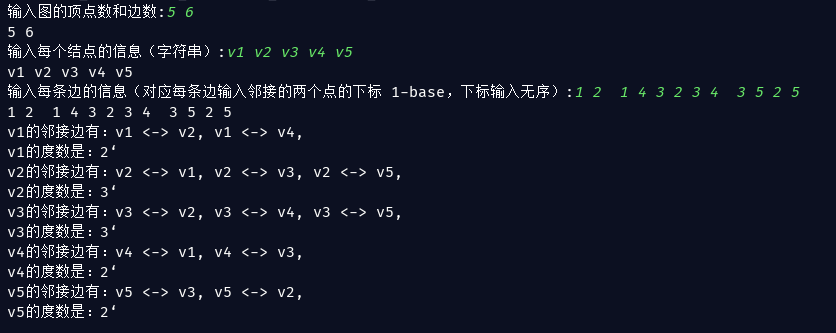
\includegraphics[width=0.6\linewidth]{1.PNG}
        \caption{栈的构造,析构,pop,push,top功能实现}
      \end{figure}

\subsection{项目2}
大致思想 :顺序存储,利用一个数组存储队列中的数,标记队首(front)和队尾(rear)的位置。push back:  rear++, pop front:  front++;节省空间。Q.base[Q.rear]=d; Q.rear = (Q.rear+1)\%MAXSIZE;对MAXSIZE 取余,保证了 rear 的最大值永远不会超过容量。注意front=rear 不能区分队列 empty 还是 full,所以少用一个空间存储数字,即当front = rear+1  is full; 
\subsubsection{实验步骤}
\begin{enumerate}
\item 构造initeQueue()函数,只需要为数组开辟一片空间,初始化rear 和 front,复杂度O(1);
\item 析构为了和项目1隐式析构区别,现写显式调用的析构函数DestroyQueue,只需释放数组空间,初始化rear front,复杂度O(1);
\item queueSize,利用(Q.rear-Q.front+MAXSIZE)\%MAXSIZE直接计算,复杂度O(1);
\item EnQueue,新元素只需要在队尾入队列,若队满调整MAXSIZE,复杂度O(1);
\item DeQueue,调整队首,front++,再对MAXSIZE取余,保证值始终在数组下标内范围,复杂度O(1);
\item isEmpty函数  由于判full有(size+1=MAXSIZE),不会与判empty(rear=front)重复,直接根据第一个if判断,复杂度O(1);
\item print 函数,需要遍历一遍输出,复杂度O(n)(n为队列元素个数);
\end{enumerate}
\subsubsection{必要代码}
\lstinputlisting[language=C++]{code/2.cpp}
\subsubsection{实验结果}见下图2
	\begin{figure}[!bthp]
	\centering
        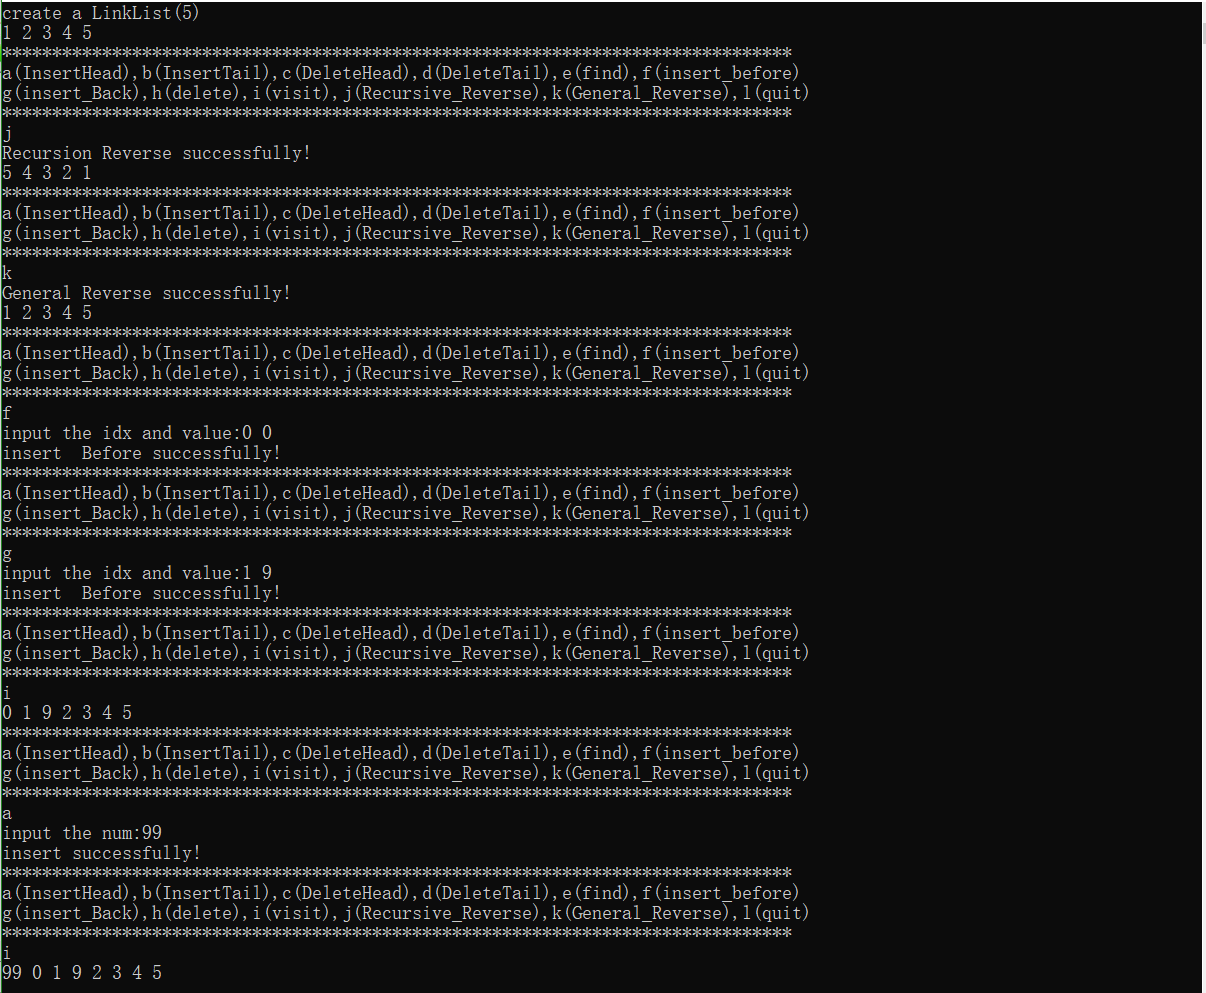
\includegraphics[width=0.6\linewidth]{2.PNG}
        \caption{队列的析构,构造,出入队,size,isEmpty()等基本操作}
      \end{figure}


\subsection{项目3}
大致思想:利用栈结构特点存储计算后缀表达式,逐个读入字符,遇到数字就入栈,遇到计算符就pop出俩栈顶元素,并用这个运算符计算,再将结果push入栈,读入下一个字符。读完字符串后,取出栈顶元素,即最后结果。 
\subsubsection{实验步骤}
\begin{enumerate}
\item compute函数,判定运算符进行相应的计算,复杂度O(1);
\item TransCharToNum函数,将数字字符转换成真正的数字,复杂度O(1);
\item main函数,逐个遍历读入字符串,计算sum,复杂度O(n)(n为字符串长度);
\end{enumerate}
\subsubsection{必要代码}
\lstinputlisting[language=C++]{code/3.cpp}
\subsubsection{实验结果}见图3
	\begin{figure}[!bthp]
	\centering
        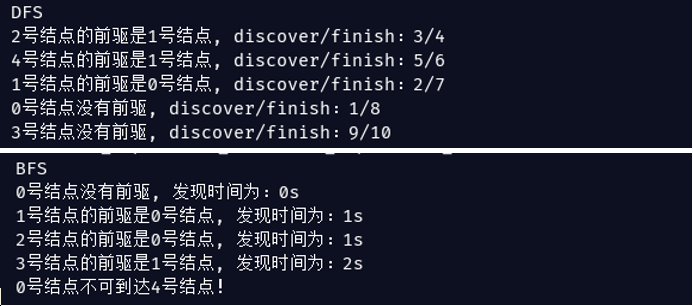
\includegraphics[width=0.6\linewidth]{3.PNG}
        \caption{利用栈的结构计算后缀表达式}
      \end{figure}


\subsection{项目4.1}
大致思想:利用栈结构特点存储自定义优先级的运算符,逐个读入字符串,遇到数字就打印,遇到非数字判断优先级,决定出入栈,注意实验步骤中描述的涉及到的用户输入容错处理。
\subsubsection{实验步骤}
\begin{enumerate}
\item 开头遇到正号无实际意义,直接跳过,遇到负号代表接下来的数字是个负数,直接打印,不归入运算符内;
\item 后缀表达式中间夹杂空格,跳过
\item 若遇到+-,--,*-,/-,(-,代表当前a[i]=‘-’后的数字为负数,直接输出符号,不是运算符
\item 若遇到)+,空格+等一系列非数字后面接+号的情况,正号冗余,跳过;
\item main函数内,真正处理运算符时,依照上述优先级判断入栈还是出栈,遍历一遍循环n次,循环内部判断优先级,pop直到优先级相对大小变化时,最坏循环n次,综上,复杂度O($n^2$)(n为字符串长度)
\end{enumerate}
\subsubsection{必要代码}
\lstinputlisting[language=C++]{code/4-1.cpp}
\subsubsection{实验结果}见图4
	\begin{figure}[!bthp]
	\centering
        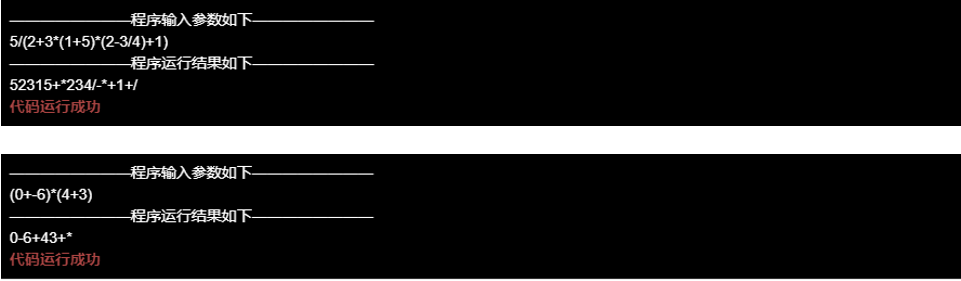
\includegraphics[width=0.6\linewidth]{4-1.PNG}
        \caption{中缀表达式转换成后缀表达式}
      \end{figure}

\subsection{项目4.2}
即项目三


\subsection{项目4.3}
大致思想:括号匹配属于经典栈的应用。逐个遍历字符串,但凡是左括号,为等待右括号匹配的待定项,入栈;若为右括号,与栈顶元素匹配,不匹配,本次检验失败,匹配,左括号出栈,进行下一轮读取。若栈空,没能匹配得到,匹配失败。遍历结束,栈空,说明都匹配成功。否则是匹配失败
\subsubsection{实验步骤}
\begin{enumerate}
\item main函数,只需逐个遍历一次字符串,判断匹不匹配,复杂度O(n)(n为字符串长度);
\end{enumerate}
\subsubsection{必要代码}
\lstinputlisting[language=C++]{code/4-3.cpp}
\subsubsection{实验结果}见图5     
	\begin{figure}[!bthp]
	\centering
        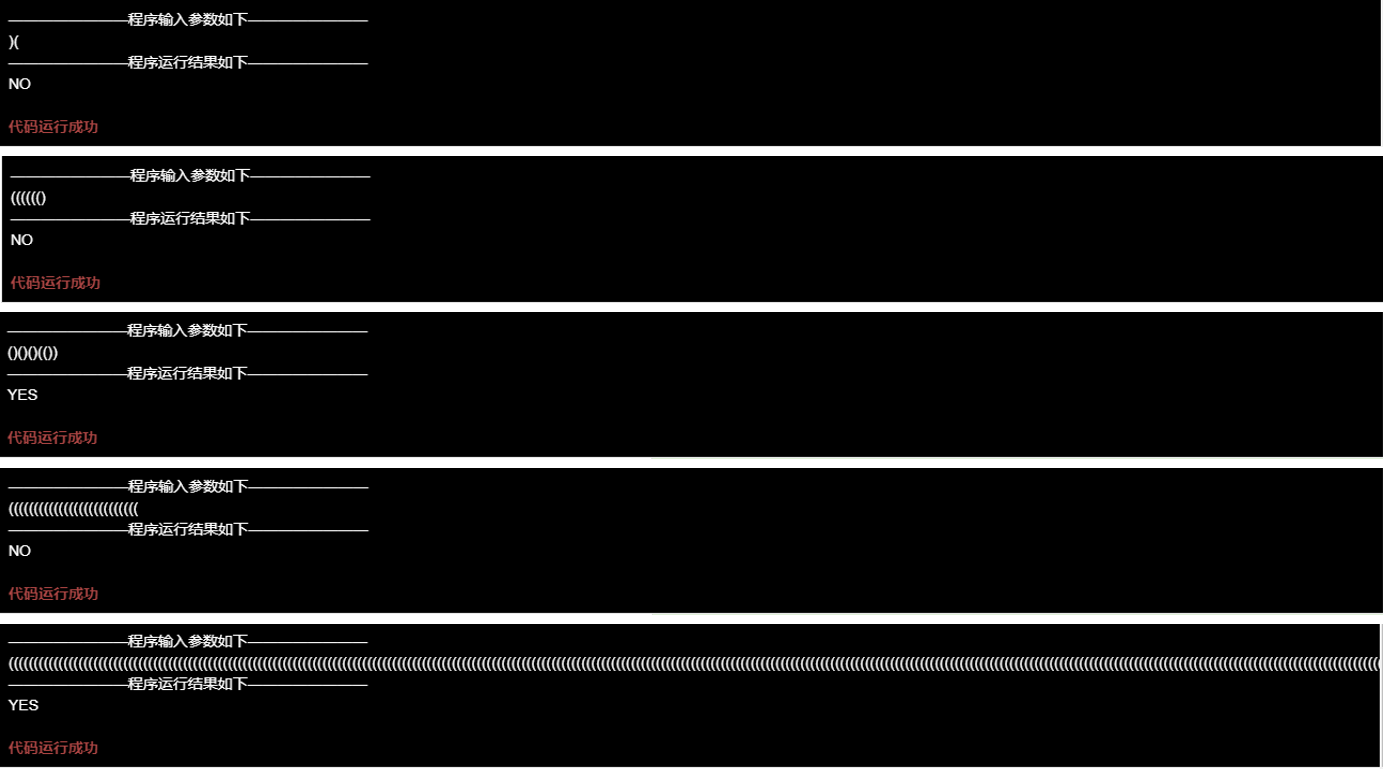
\includegraphics[width=0.6\linewidth]{4-3.PNG}
        \caption{栈的应用之括号匹配}
      \end{figure}

\subsection{项目4.4}
大致思想:利用栈结构后进先出的特点存储转换过来的n进制数的每一位数,再逐个打印出栈顶元素和pop,出来的顺序即进制转换的结果。
\subsubsection{实验步骤}
\begin{enumerate}
\item conversion函数,对十进制数累除,复杂度O($log_n num$),其中n为进制,num为十进制数;
\end{enumerate}
\subsubsection{必要代码}
\lstinputlisting[language=C++]{code/4-4.cpp}
\subsubsection{实验结果}见图6
	\begin{figure}[!bthp]
	\centering
        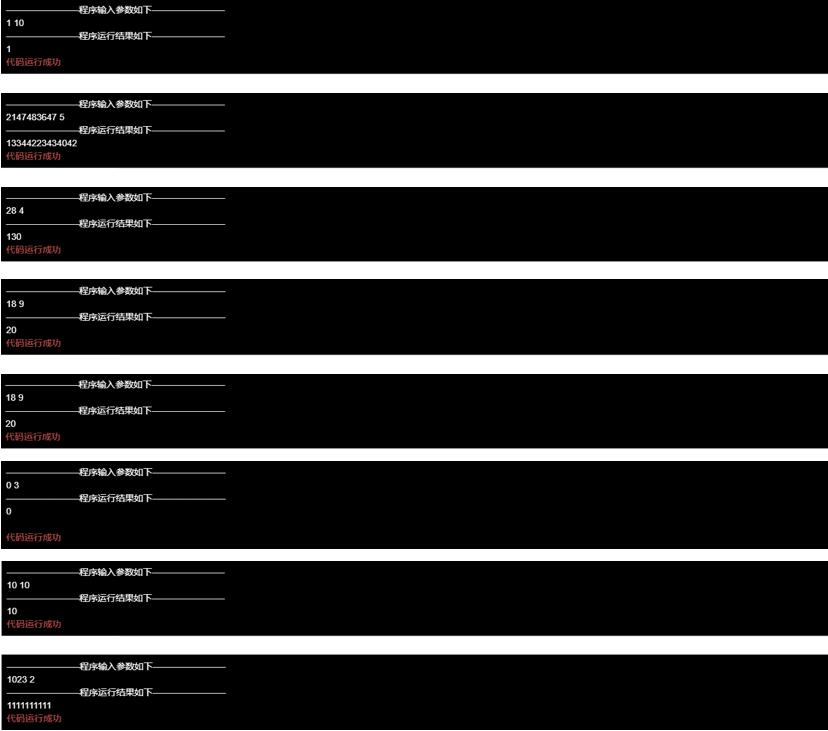
\includegraphics[width=0.6\linewidth]{4-4.PNG}
        \caption{栈的应用之进制转换}
      \end{figure}




\section{实验总结}
\begin{enumerate}
\item 进步:掌握栈和队列的基本操作(特别地,巩固了析构函数和循环队列的知识),掌握栈的三种应用:计算后缀表达式,进制转换,括号匹配。
\item 不足:程序设计考虑不周全,不能一次性考虑周全所有情况;细节(尤其是链表操作头尾指针的单独处理操作)缺乏把控!
\end{enumerate}
\end{document}
